\documentclass[border=10pt]{standalone}
\usepackage{xcolor}
\usepackage{pgfplots}
\usepackage{tikz}
\begin{document}
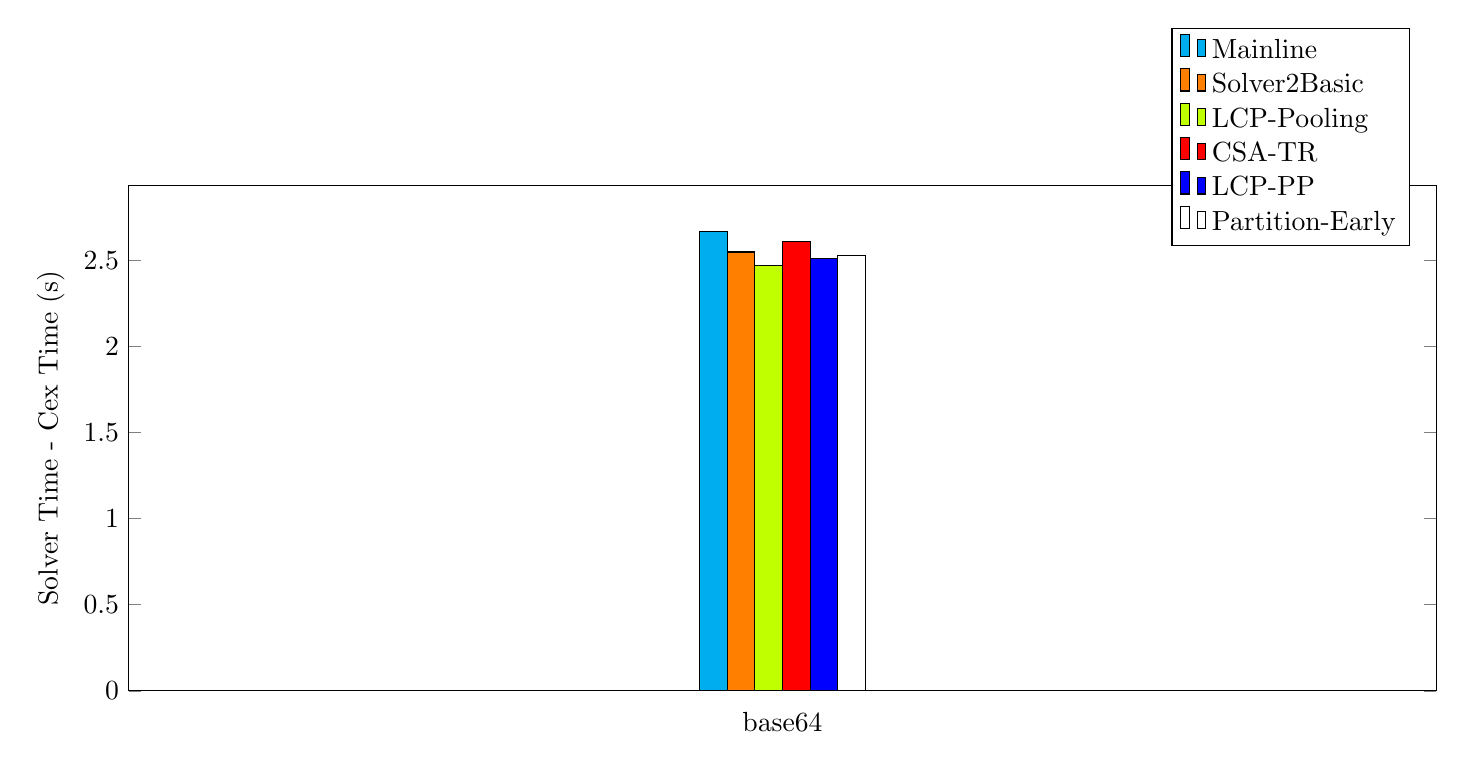
\begin{tikzpicture}
    \begin{axis}[
        width  = 1.5 * \textwidth,
        height = 8cm,
        major x tick style = transparent,
        % tickwidth=10,
        ybar=0,
        bar width=10pt,
        % ymajorgrids = true,
        ylabel = {Solver Time - Cex Time (s)},
        symbolic x coords={base64},
        xtick = data,
        scaled y ticks = false,
        enlarge x limits=0.05,
        ymin=0,
        legend cell align=left,
        legend style={
                at={(0.98,0.88)},
                anchor=south east,
                % column sep=1ex
        }
    ]
        \addplot[style={cyan,fill=cyan,mark=none}, draw=black]
	coordinates {(base64,2.6700000000000017)};
\addplot[style={orange,fill=orange,mark=none}, draw=black]
	coordinates {(base64,2.549999999999997)};
\addplot[style={lime,fill=lime,mark=none}, draw=black]
	coordinates {(base64,2.469999999999999)};
\addplot[style={red,fill=red,mark=none}, draw=black]
	coordinates {(base64,2.6099999999999994)};
\addplot[style={blue,fill=blue,mark=none}, draw=black]
	coordinates {(base64,2.510000000000005)};
\addplot[style={white,fill=white,mark=none}, draw=black]
	coordinates {(base64,2.530000000000001)};

        \legend{Mainline,Solver2Basic,LCP-Pooling,CSA-TR,LCP-PP,Partition-Early}
    \end{axis}
\end{tikzpicture}
\end{document}
